\documentclass[letterpaper, 12pt]{article}

\usepackage{geometry}
 \geometry{
 letterpaper,
 total={170mm,257mm},
 left=20mm,
 top=20mm,
 bottom=20mm
 }
\usepackage{graphicx} % Required for inserting images
\usepackage{authblk}
\usepackage{amssymb}
\usepackage{lipsum}
\usepackage{float}
\usepackage{times}
\usepackage{amsmath}
\usepackage[format=plain,
            labelfont={bf,it},
            textfont=it]{caption}
\captionsetup{justification=raggedright,singlelinecheck=false}
\usepackage{ragged2e}
\usepackage{longtable}
\usepackage{comment}
\usepackage{setspace}
\usepackage{fancyhdr}
\usepackage{titlesec}
\usepackage[hyperindex,breaklinks]{hyperref}
\hypersetup{
    colorlinks=true,
    linkcolor=blue,
    filecolor=magenta,      
    urlcolor=blue,
    pdftitle={Overleaf Example},
    pdfpagemode=FullScreen,
    }
% \usepackage{background} % add COSIG logo to page
\usepackage[T1]{fontenc}
\usepackage{helvet}
\renewcommand{\familydefault}{\sfdefault}
\pagenumbering{gobble}
\usepackage[skip=10pt plus1pt, indent=40pt]{parskip}

\titlespacing*{\section}
{0pt}{1.5ex plus 1ex minus .2ex}{1.3ex plus .2ex}

\renewcommand\Authfont{\fontsize{12}{14.4}\selectfont}
\renewcommand\Affilfont{\fontsize{9}{10.8}\itshape}
 
\begin{document}
\flushleft

\includegraphics[width=0.5\textwidth]{img/home/241017_final_logo_mockup.png}

\section*{Nucleotide sequence reagents}
\addcontentsline{toc}{section}{Nucleotide sequence reagents}
\textit{Last updated: 28 March 2025}

Nucleotide sequence reagents, short strands of DNA or RNA, are frequently used in a variety of biomedical experiments. Because the sequence of base pairs that compose a nucleotide sequence reagent are \href{https://doi.org/10.1373/clinchem.2008.112797}{expected to be} specified in the text of an article and because the genomes of most organisms used in these experiments are well-characterized, nucleotide sequence reagents are readily verifiable. In other words, most nucleotide sequence reagents can be fact-checked to ensure that they would work as described.

\subsection*{Types of nucleotide sequence reagents}

\subsubsection*{PCR primers}

\subsubsection*{RT-qPCR primers}

\subsubsection*{siRNA}

\subsubsection*{shRNA}

\subsection*{Example section heading}

\subsection*{Checking nucleotide sequences}

\subsection*{Example 1:}

\begin{figure}[h!tbp]
    \centering
    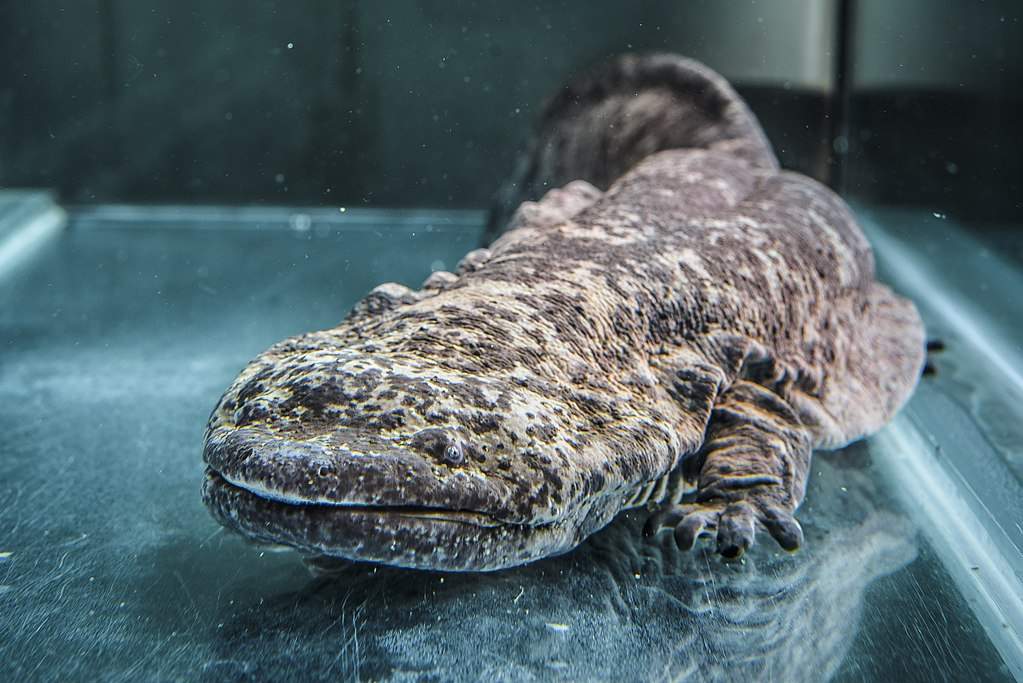
\includegraphics[width=0.8\textwidth]{img/home/chinese_giant_salamander.jpg}
    \caption*{Example of a figure. Image available \href{https://commons.wikimedia.org/wiki/File:Velemlok_\%C4\%8D\%C3\%ADnsk\%C3\%BD_zoo_praha_1.jpg}{here}.}
\end{figure}

\begin{itemize}
    \setlength\itemsep{-0.5em}
    \item bullet
    \item point
    \item list
\end{itemize}

\begin{enumerate}
    \setlength\itemsep{-0.5em}
    \item numbered
    \item list
\end{enumerate}

\pagebreak

If there is a large block of quoted text, use:

\begin{quote}
    \textit{Note that this text is in italics!}
\end{quote}

When linking out to articles using \verb|\href|, try to use the DOI instead of a link to the publisher site or PubMed page.

\end{document}